\usetikzlibrary{arrows}
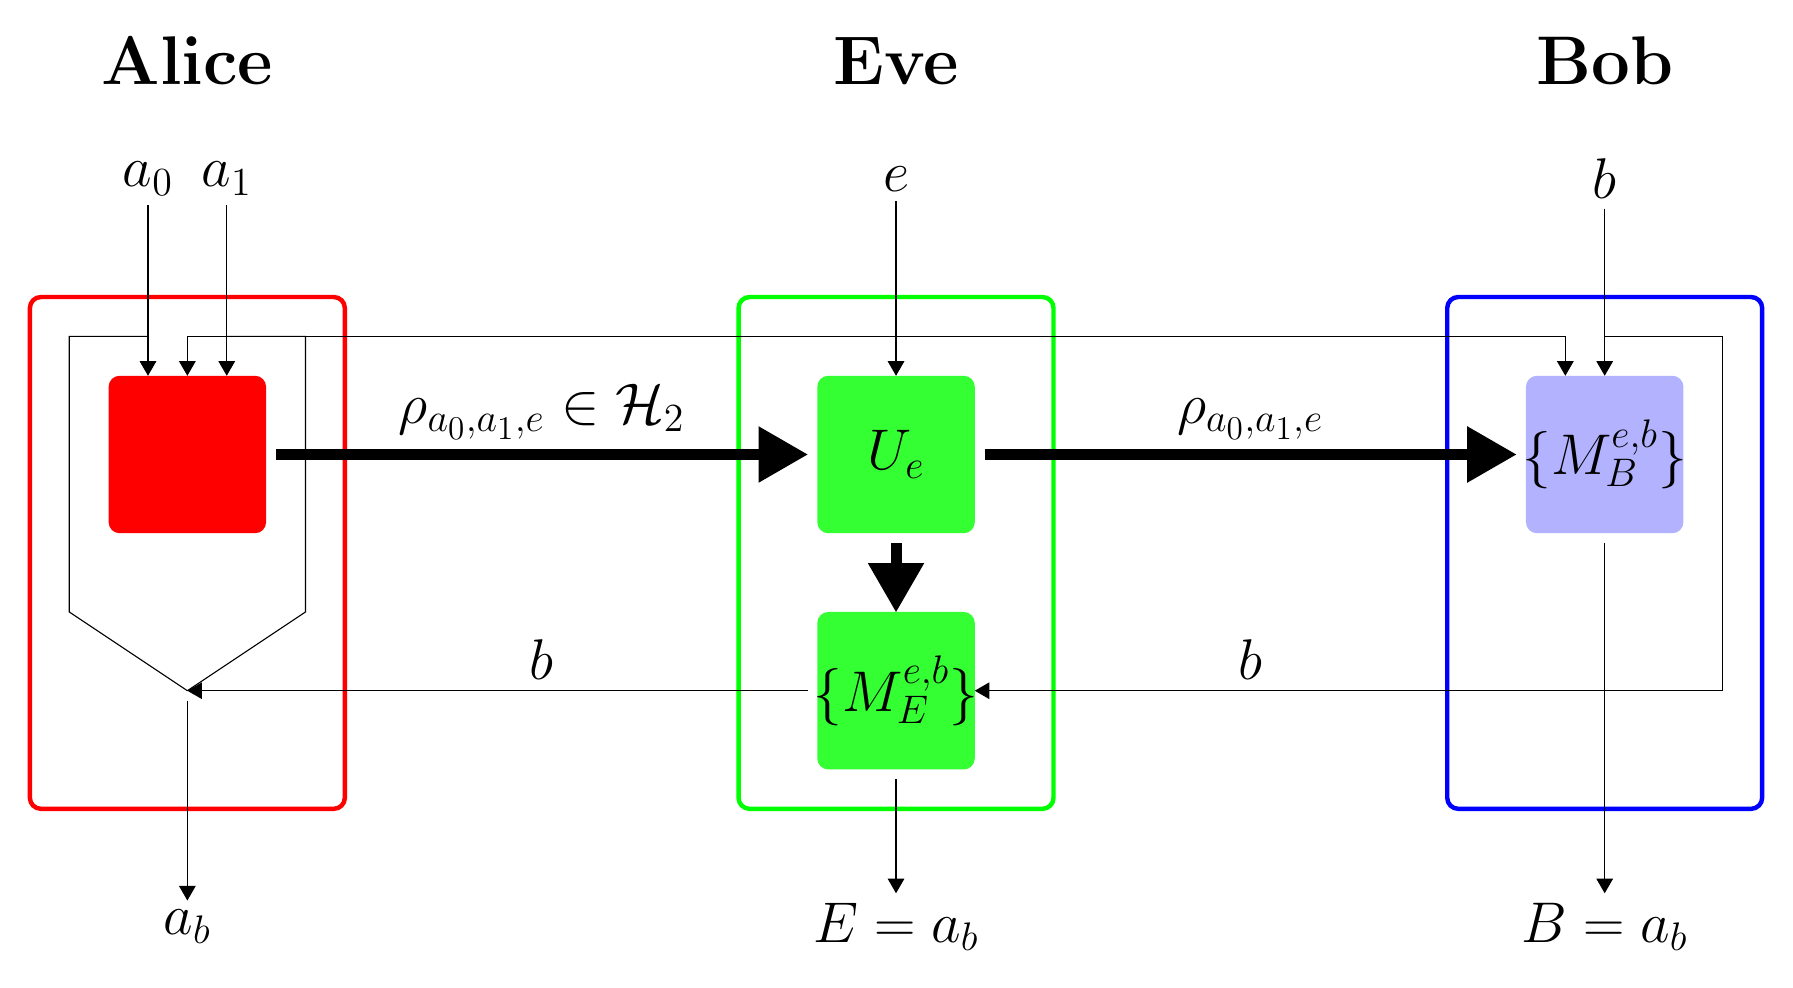
\begin{tikzpicture}

\fill[rounded corners,color=red]  (-4,2.5) rectangle (-2,0.5);
\fill[rounded corners,color=green,opacity=0.8]  (5,2.5) rectangle (7,0.5);

\node at (-2.5,2) {};
\coordinate (v6) at (6,2.5) {};
\node (v7) at (6,-2.5) {};
\node (v1) at (-3.5,5) {\huge $a_0$};
\node (v3) at (-2.5,5) {\huge $a_1$};
\node (v5) at (6,5) {\huge$e$};
\node (v8) at (6,-4.5) {\huge $E=a_b$};
\node (v19) at (-2,1.5) {};
\draw[rounded corners,color=red,ultra thick]  (-5,3.5) rectangle (-1,-3);
\draw[rounded corners,color=green,ultra thick]  (4,3.5) rectangle (8,-3);
\coordinate (v2) at (-3.5,2.5) {};
\coordinate (v4) at (-2.5,2.5) {};
\draw [o-*, -triangle 60] (v1) edge (v2);
\draw [o-*, -triangle 60] (v3) edge (v4);
\draw [o-*, -triangle 60] (v5) edge (v6);
\draw [o-*, -triangle 60] (v7) edge (v8);
\coordinate (v9) at (-3.5,3) {};
\coordinate (v10) at (-4.5,3) {};
\coordinate (v11) at (-4.5,-0.5) {} {};
\coordinate (v16) at (-1.5,3) {};
\coordinate (v15) at (-2.5,3) {};
\coordinate (v17) at (-1.5,-0.5) {} {};
\coordinate (v12) at (-3,-1.5) {} {} {} {} {} {};
\node (v13) at (-3,-1.5) {};
\node (v14) at (-3,-4.5) {\huge $a_b$};
\coordinate (v18) at (16.5,-1.5) {};

\draw (v9) -- (v10) -- (v11) -- (v12) -- (v13);
\draw (v15) -- (v16) -- (v17) -- (v12);
\draw [-triangle 60] (v13) edge  (v14);
\node (v20) at (5,1.5) {};
\draw [-triangle 60,line width=4pt] (v19) edge node[above]{\huge $\rho_{a_0,a_1,e}\in \mathcal{H}_2$} (v20);
\node at (-3,6.5) {\Huge \bf Alice};
\node at (6,6.5) {\Huge \bf Eve};
\draw[rounded corners,color=blue,ultra thick]  (13,3.5) rectangle (17,-3);
\coordinate (v21) at (6,3) {};
\coordinate (v22) at (-3,3) {};
\coordinate (v23) at (-3,2.5) {};
\draw [-triangle 60] (v21) -- (v22) -- (v23);
\fill[rounded corners,color=blue,opacity=0.3]  (14,2.5) rectangle (16,0.5);
\node (v26) at (15,5) {\huge $b$};
\coordinate (v27) at (15,2.5) {};
\coordinate (v25) at (14.5,2.5) {};
\coordinate (v24) at (14.5,3) {};
\draw [-triangle 60] (v21) -- (v24) -- (v25);
\draw [-triangle 60] (v26) edge (v27);
\coordinate (v28) at (15,3) {};
\coordinate (v29) at (16.5,3) {};
\node (v30) at (15,0.5) {};
\node (v31) at (15,-4.5) {\huge $B=a_b$};
\node at (15,6.5) {\Huge \bf Bob};
\draw [-triangle 60] (v30) edge (v31);
\node (v32) at (7,1.5) {};
\node (v33) at (14,1.5) {};
\draw [-triangle 60,line width=4pt]  (v32) edge node[above]{\huge $\rho_{a_0,a_1,e}$} (v33);
\node at (6,1.5) {\huge $U_e$};
\node at (15,1.5) {\huge $\{M_B^{e,b}\}$};
\fill[rounded corners,color=green,opacity=0.8]  (5,-0.5) rectangle (7,-2.5);
\node (v34) at (6,0.5) {};
\coordinate (v35) at (6,-0.5) {};
\draw [-triangle 60,line width=4pt]  (v34) edge (v35);
\node at (6,-1.5) {\huge $\{M_E^{e,b}\}$};
\coordinate (v36) at (7,-1.5) {};
\draw [-triangle 60](v28) -- (v29) -- (v18) -- (v36);
\node (v37) at (5,-1.5) {};
\draw [-triangle 60] (v37) edge (v12);
\node at (10.5,-1-0.1) {\huge $b$};
\node at (1.5,-1-0.1) {{\huge $b$}};
\end{tikzpicture}